% This is samplepaper.tex, a sample chapter demonstrating the
% LLNCS macro package for Springer Computer Science proceedings;
% Version 2.20 of 2017/10/04
%
\documentclass[runningheads]{llncs}
%
\usepackage{graphicx}
% Used for displaying a sample figure. If possible, figure files should
% be included in EPS format.
%
% If you use the hyperref package, please uncomment the following line
% to display URLs in blue roman font according to Springer's eBook style:
% \renewcommand\UrlFont{\color{blue}\rmfamily}

\begin{document}
%
\title{Admission Handler}

\author{Group 18: Jan Haas \and Simon Hauser \and Sam Kenworthy}

\institute{}
%
\maketitle              % typeset the header of the contribution

\section{Introduction}
This project implements a distributed admission system for large events and venues with limited capacity.
The stream of visitors entering or exiting the venue will be monitored in real-time via devices at each entrance.
Live feedback will be provided to each device, enabling organizers to stop admission when the maximum capacity of the venue has been reached.

As the world starts to reopen after the pandemic and public events become possible again, systems are required to handle the keeping of safe capacities, in-line with changing guidelines and laws.
Pre-selling tickets is one possibility of managing these limits, yet events such as Christmas markets, beer gardens and public concerts live off spontaneous visits.
This project will enable the simple monitoring and managing of such streams of visitors, by providing a dynamically scalable system.

\section{Requirements Analysis}
\subsubsection{Dynamic Discovery}
A fresh server joins the system by broadcasting a join request.
If it does not receive answers, it establishes itself as the new system with zero current guests.
If it does get an answer, the number of arrivals is synchronized between servers.
New clients join the system by broadcasting a request and establishing a TCP connection with the first server to answer them.

\subsubsection{Ordered Reliable Multicast}
Clients communicate newly arriving guests to their server and only allow passage if they get a positive response.
To ensure a fair entry process and for possible other uses, arrivals are causally ordered.
This is achieved by sending the entry request to the other servers using reliable ordered multi-cast.
New arrivals are only permitted if they have been integrated in the causal order and are not over capacity according to it.
New entries are also communicated to all connected clients to ensure they display correctly how many free spots are left.

\subsubsection{Voting}
The servers establish a leader that manages the group view and decides in the case of disputes over the correct order of entries, if they can occur (how exactly it will do that is currently yet unclear to us).
To ensure that a recovery process can be started early, the leader sends periodic life signs to each server in the group and starts the recovery process if there is no answer (from one of the servers).

\subsubsection{Fault Tolerance}
If a client does not receive an answer from its associated server, it tries to find a new one via the same process as a freshly joining one.
If a server does not hear from a client, the TCP connection is simply purged.
Each of the servers keeps the order (and number) of entries in memory so it can take over in case the leader fails.
If a server loses an established connection to a system, it notifies connected clients and goes dormant until it is able to reestablish the connection.
This ensures that the venue does not go over capacity from having two independent systems exist.
From the system side, if a single server cannot be reached anymore, other servers simply close the connection to it.
If the leader loses connection, the other servers elect a new one after receiving no pings from it but still having a connection to each other, which they check via using a broadcast.
\section{Architecture}
The system will be modeled in a single network with at least a machine running multiple clients and at least two running some servers each.
Both participant types will be written in Python.\\
\begin{figure}
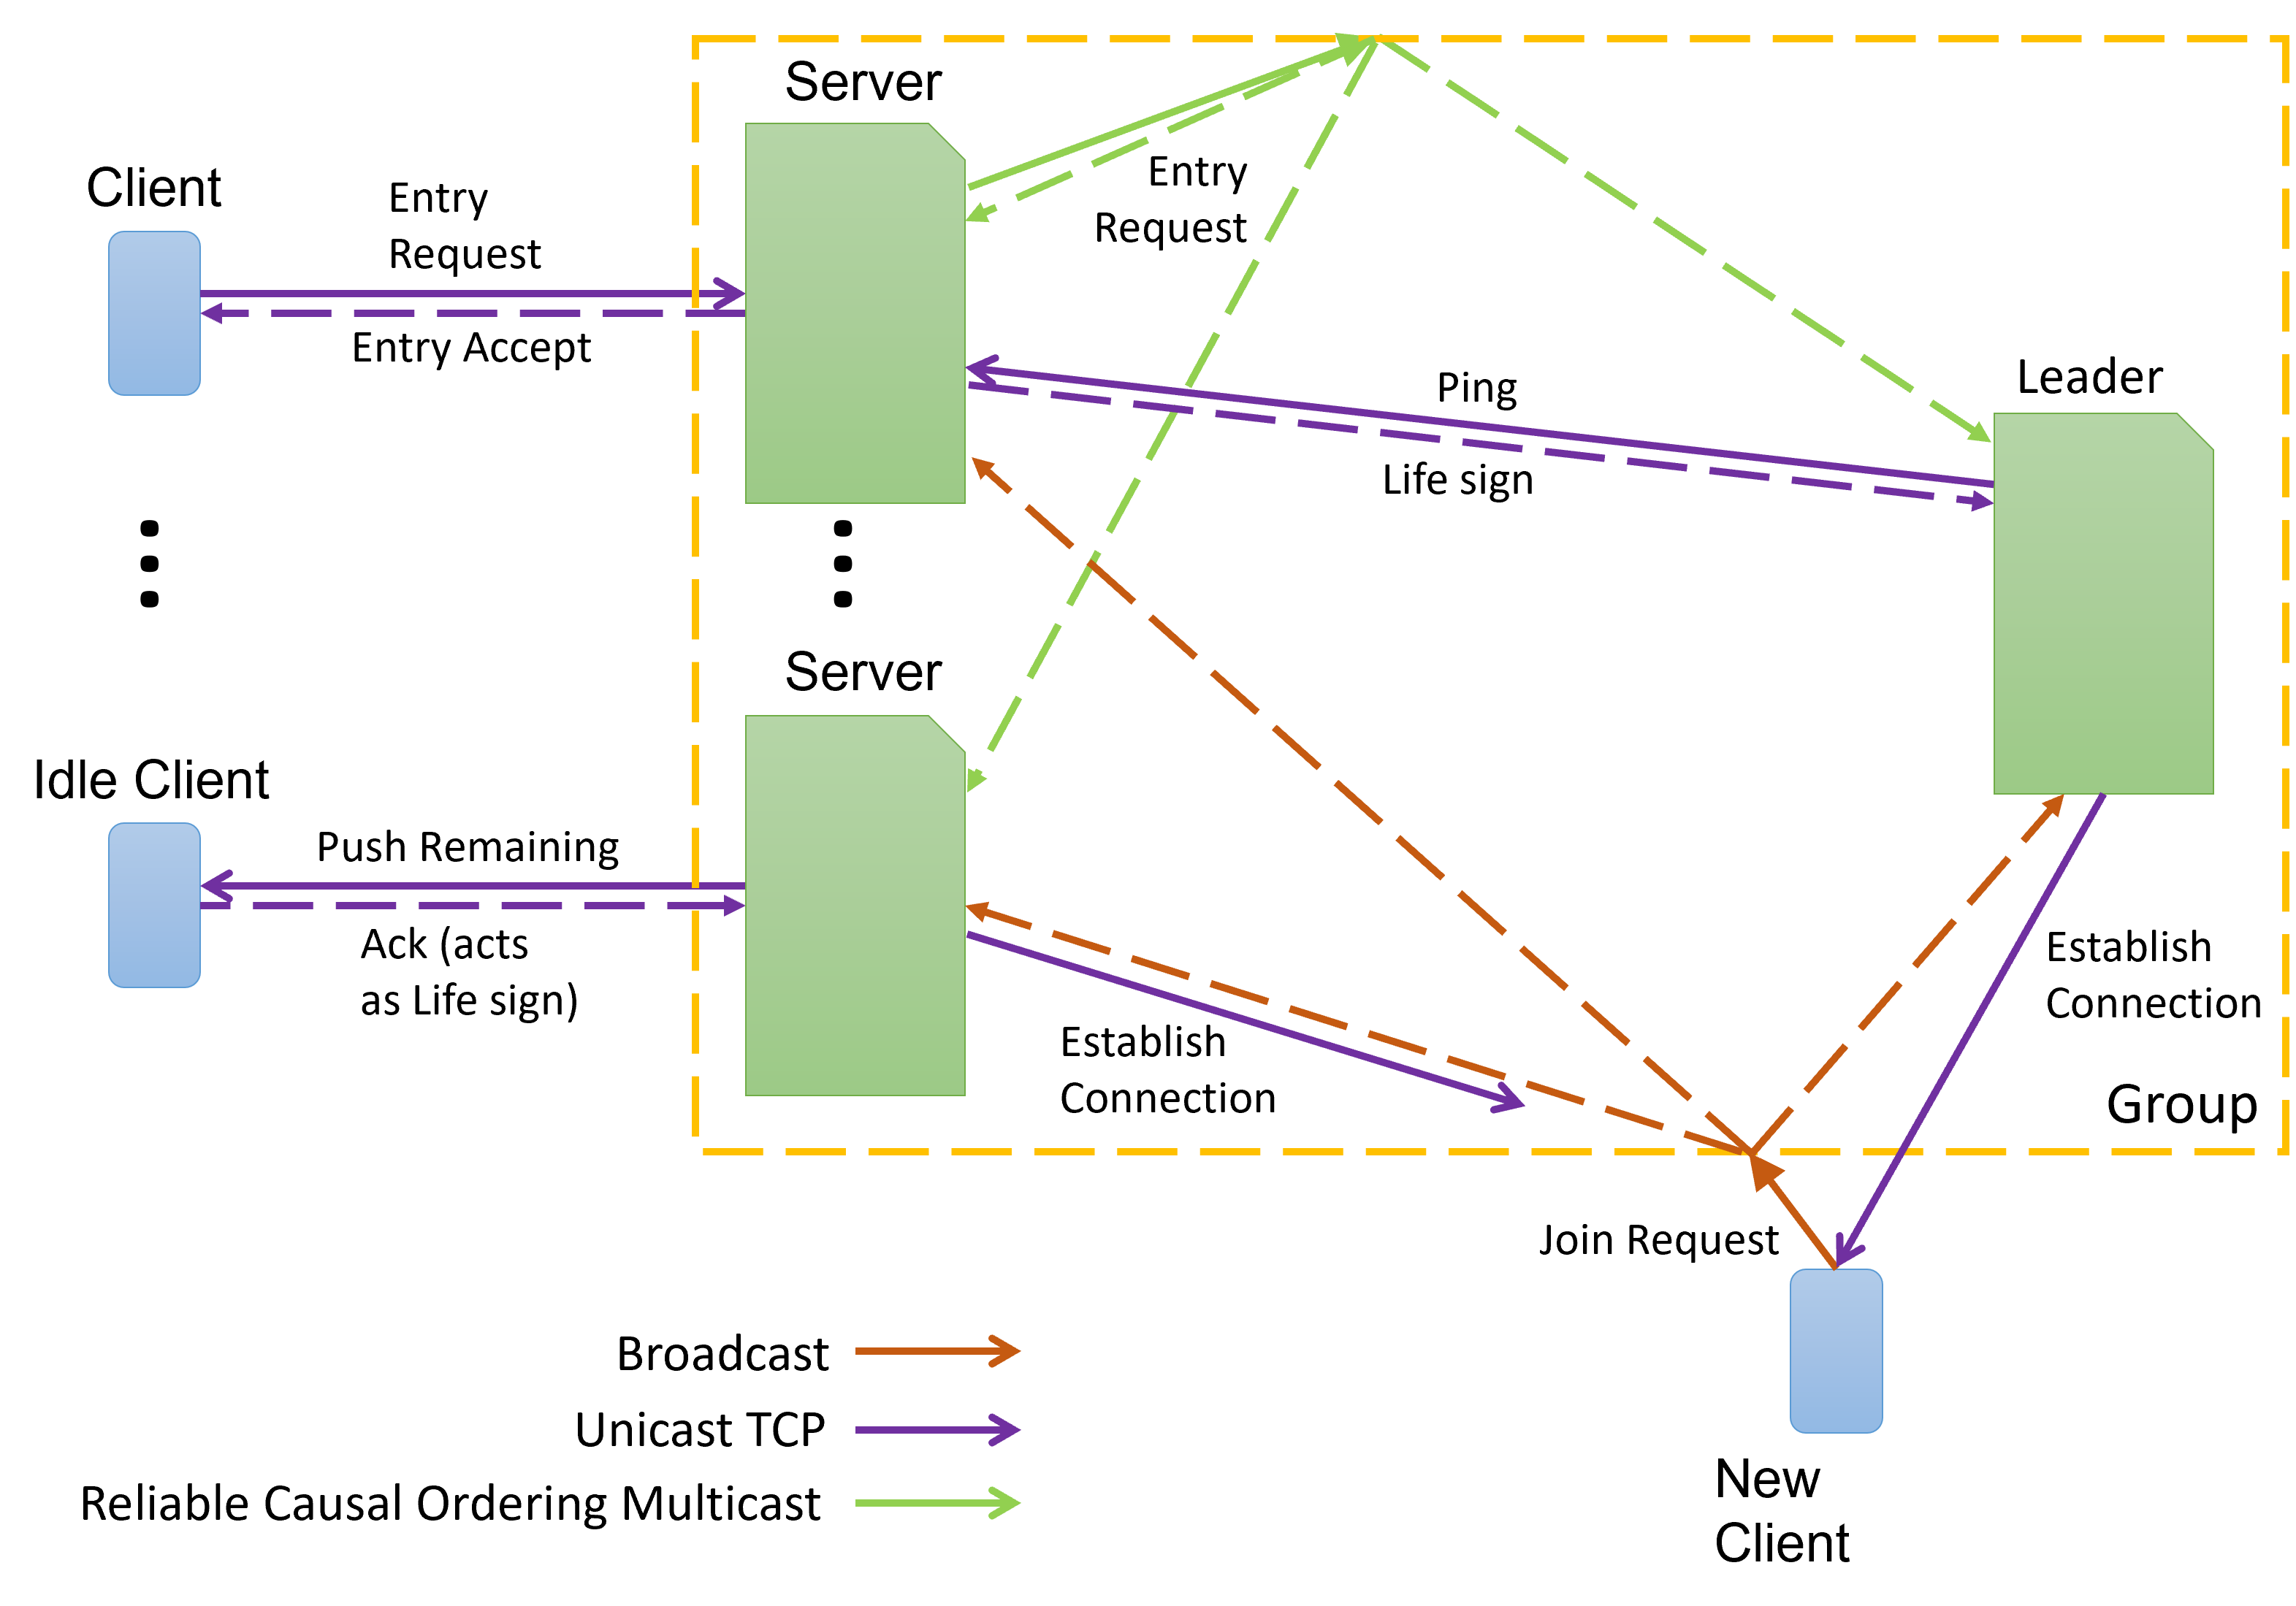
\includegraphics[width=\textwidth]{Architecture_Diagram.png}
\end{figure}
\end{document}
